\documentclass{beamer}
\setbeamertemplate{navigation symbols}{}
\usetheme{Malmoe}
\usecolortheme{beaver}
%\usepackage{natbib}   
%\bibliographystyle{plainnat}
\bibliographystyle{apalike}   % Or any other style you like
%\bibliographystyle{natbib} % kürzt automatisch vornamen ab und so zeug 
%\beamertemplatenavigationsymbolsempty
\beamersetuncovermixins{}{}
%\setbeamercovered{invisible}
%\usepackage{float}
\usepackage{amssymb}
\usepackage{wrapfig}
\usepackage{amsmath}
\usepackage[english]{babel}
\usepackage[utf8]{inputenc}
\usepackage{float}
\usepackage{graphicx}
%\usepackage{wrapfig}
\usepackage{textcomp}
\usepackage{braket}
\usepackage{bbm}
\usepackage{framed}
\usepackage{ifthen}
\usepackage{bbold}
\usepackage{colortbl}
\usepackage{xifthen}
\usepackage{color}
\usepackage{ifthen}
\usepackage[T1]{fontenc}
\usepackage{amsthm}
\usepackage{bm}
\usepackage{amsbsy}
\usepackage{tikz}
\usepackage{nicefrac}
\usepackage{chessboard, xskak}
\usepackage{xspace}

\usepackage{xcolor}
\usepackage{scalefnt}
\usepackage{caption}
\addto\captionsngerman{
\renewcommand{\figurename}{Figure}%
\renewcommand{\tablename}{Tab.}%
}
\setlength{\parskip}{1.5ex plus0.5ex minus0.5ex}
\setlength{\parindent}{0em} 

\sloppy \frenchspacing \raggedbottom 


\usetikzlibrary{trees}
\usetikzlibrary{positioning}
\tikzset{main node/.style={circle,fill=black,draw,minimum size=3pt,inner sep=0pt},}
\tikzset{
    invisible/.style={opacity=0,text opacity=0},
    visible on/.style={alt=#1{}{invisible}},
    alt/.code args={<#1>#2#3}{%
      \alt<#1>{\pgfkeysalso{#2}}{\pgfkeysalso{#3}} 
    },
    beameralert/.style={alt={<#1>{fill=red!30,rounded corners}{}},anchor=base},
    BeamerAlert/.style={alt={#1{fill=red!30,rounded corners}{}},anchor=base}
}
  \newcommand<>{\tikzMe}[1]{% previously: \def\tikzMe<#1>#2{…
    \tikz[baseline]\node[BeamerAlert={#2},anchor=base] {#1};
}

%\usetikzlibrary{external}
%\tikzexternalize[prefix=external]
\usepackage{verbatim}

\newcommand{\V}{\ensuremath{\mathbf{V}}\xspace}
\newcommand{\F}{\ensuremath{\mathbf{F}}\xspace}


\newcommand\blfootnote[1]{%
  \begingroup
  \renewcommand\thefootnote{}\footnote{#1}%
  \addtocounter{footnote}{-1}%
  \endgroup
}

% Prov makro
\DeclareMathOperator*{\Prov}{Prov}
\DeclareMathOperator*{\Var}{Var}

\DeclareMathOperator*{\Proov}{Proof}

\newcommand{\NP}{\ensuremath{\mathcal{NP}}}
\begin{document}
\title{Complexity Theory \& Philosophy}
\author{Abraham Hinteregger}
\institute{Vienna University of Technology}
\date{2016-06-27}
\titlepage
\setcounter{tocdepth}{3}
\AtBeginSection[]{
\begin{frame}
\frametitle{Chapter} 
\tableofcontents[currentsection,currentsubsection,hideothersubsections]
\end{frame}
}

\setbeamertemplate{footline}[frame number]
\section{Complexity Theory}
\subsection{Introduction}

\begin{frame}{Some historical background}
\begin{itemize}
\item 85 years ago Gödel introduced incompleteness theorems\footnote{\cite{goedel1}}
\item 5 years later Turing generalized this to limitations of computation (Halting)\footnote{\cite{turing}}
\item When ``computing machines'' became reality, time and space requirements of algorithms were of interest \footnote{\cite{complex1}: On the comp. complexity of algorithms}
\end{itemize}
\end{frame}




%\begin{frame}{Overview}
%\begin{itemize}
%\item TODO difference time \& space, reusability
%
%\end{itemize}•
%\end{frame}

\subsection{Computability \& Complexity}
\begin{frame}{Computability vs. Complexity}
\begin{itemize}
\item<1-> Difference between something being \textit{computable} or \textit{uncomputable} obviously of philosophical importance
\item<1-> What about \textit{computable} and \textit{efficiently computable}?
\item<2-> 10 seconds versus 20 seconds?

\only<1-4>{\uncover<3-4>{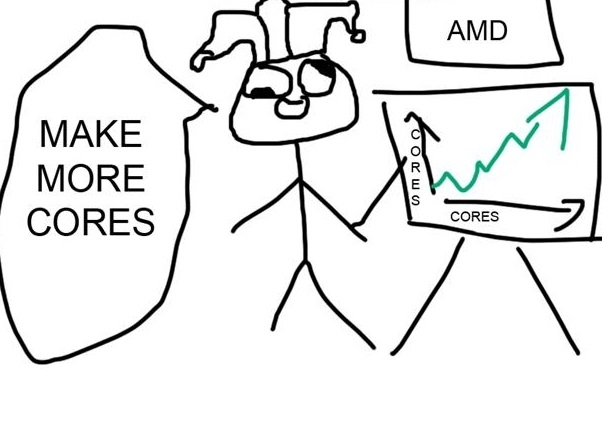
\includegraphics[width=0.44\textwidth]{img/amd0.jpg}\quad\uncover<4>{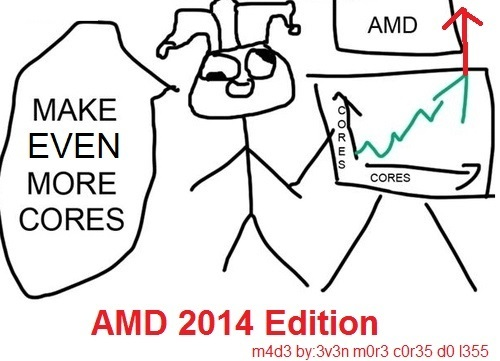
\includegraphics[width=0.44\textwidth]{img/amd1.jpg}}}}
\begin{itemize}
\item<5-> Buy more RAM/CPUs
\item<6-> Use GPUs
\item<7-> Hire TU graduates
\end{itemize}
\item<8-> Optimizing constant factors/reducing exponent concern of engineers
\item<9-> What about $100$ seconds  versus $2^{100}$ seconds? 
\begin{itemize}
\item<10-> Multiplication vs. prime factoring
\item<10-> Reading a book with 400 pages vs. reading all possible 400p books
\end{itemize}
\end{itemize}
\end{frame}

\subsection{Polynomial time}
\begin{frame}{Relevance of polynomial time}
\begin{itemize}
\item Computability Theory: Truncated HALTING problem\blfootnote{Mentioned in a letter from Gödel to von Neumann in 1956}\\[15pt]
\begin{quote}
Is there an F-proof of $S$ in $n$ or fewer symbols?
\end{quote}	
\item Decidable by exponential bruteforce algorithm
\item If there was a polynomial (with sane constants and exponent) algorithm Hilbert's dream (almost) possible
\end{itemize}
\end{frame}

\begin{frame}{Relevance of polynomial time II}
\begin{itemize}
\item Number Theory: largest ``known'' prime: $p = 2^{74,207,281}-1$
\begin{itemize}
\item expression picks out unique positive integer
\item that integer has to be a prime number
\end{itemize}
\item<2-> Why $p$ and not $p' = \text{first prime s.t. } p' > p$?
\item<3-> What criterion is used to call a number a ``known prime''? 
\begin{itemize}
\item<4-> Is it possible to store the decimal expansion somewhere? Would $2^{2^{2^{1231}}}-1$ not be a known prime (if it is prime) because the universe is too small?
\item<5-> Maybe the existence of polynomial ($n$ = number of digits) procedure to output the decimal digits of $p$ would explain ``knowing''
\end{itemize}
\end{itemize}
\end{frame}


\section{Turing test \& AI}
\subsection{Turing Test}\blfootnote{\cite{turing2}}
\begin{frame}[allowframebreaks]{The Turing Test}
Evaluator converses with machine that pretends to be human and a real human. If evaluator can't distinguish the two the machine passes the test. 
\begin{itemize}
\item Additional requirements could be added, e.g.: vision, hearing, handwriting, drawing
\item The test allows a maximum amount of information to be exchanged, e.g. $2^{30}$ bits. 
\end{itemize}
\end{frame}

\begin{frame}{Chinese Room Argument}
Argument against ``strong AI'', presented by John Searle in 1980
\begin{itemize}
\item Store all things the evaluator could ask
\item Also store an answer for every possible question/statement
\item Output predefined answers for each question%\footnote{Maybe add a function that allows answering questions related to the current time}
\end{itemize}
\uncover<2->{$\implies$ Passing the Turing test is not a question of computability (as e.g. Roger Penrose argued  in \textit{The Emperor's New Mind}) but of complexity}
\end{frame}


\begin{frame}{Chinese Room Argument II}
\begin{itemize}
\item Chinese room argument initially made to counter ``Strong AI'' claim
\begin{itemize}
\item Chinese conversation
\item Person in huge library executes moves of the computer program
\end{itemize}
\item<2-> Nobody would claim that this person understands Chinese, therefore the program cannot give a computer ``mind'' or ``understanding'' either
\item<3-> Widely considered a bad argument
\item<3-> Flood of refutations inspired Pat Hayes to quip:
\begin{quote}
The field of cognitive science should be redefined as "the ongoing research program of showing Searle's Chinese Room Argument to be false"
\end{quote}
\end{itemize}
\end{frame}


\subsection{Simulating humans}
\begin{frame}{Simulating humans}
\begin{itemize}
\item<1-> Would a compact \& efficient program passing the Turing test be intelligent? If yes, is this possible?
\item<2-> Can humans solve NP-complete problems efficiently? \uncover<3->{No}
\item<4-> Humans are usually superior to machines at search problems with \textit{higher-level structure}, \textit{semantics}, \textit{global patterns} or \textit{symmetries}
\begin{itemize}
\item Proving Fermat's Last Theorem (still took us a while)
\item Pigeonhole Principle (put 1001 objects in 1000 slots)
\item Determining if a chess position is ``dead''
\end{itemize}
\end{itemize}
\end{frame}


\begin{frame}{Rybka vs Hikaru Nakamura (ICC, 3+0, 2008)\blfootnote{http://www.chessgames.com/perl/chessgame?gid=1497429}}
\centering
\definecolor{carnelian}{rgb}{0.7, 0.11, 0.11}
\newchessgame\setchessboard{markstyle=border,color=carnelian}
\only<+>{\setchessboard{markfields=f5,setfen=1b6/4kp2/p1p3p1/Pp1p1nPp/1P1PpP1P/2P1P3/K1R5/7R w - - 0 125}}
\only<+>{\setchessboard{markfields=b8,setfen=1b6/5p2/p1p1k1p1/Pp1p1nPp/1P1PpP1P/2P1P2R/2K5/1R6 w - - 98 174}}
\only<+>{\setchessboard{markfields=c4,setfen=1b6/5p2/p1p1k1p1/Pp1p1nPp/1PPPpP1P/4P2R/2K5/1R6 b - - 0 174}}
\only<+>{\setchessboard{markfields=c4,setfen=1b6/5p2/p1p1k1p1/Pp3nPp/1PpPpP1P/4P2R/2K5/1R6 w - - 0 175}}
\only<+>{\setchessboard{markfields=e1,setfen=8/4bp2/p1p3p1/Pp1n1kPp/1PpPpP1P/4P2R/1K6/4R3 b - - 15 182}}
\only<+>{\setchessboard{markfields=b4,setfen=8/5p2/p1p3p1/Pp1n1kPp/1bpPpP1P/4P2R/1K6/4R3 w - - 0 183}}
\only<+>{\setchessboard{markfields=e2,setfen=8/5p2/p1p3p1/Pp1n1kPp/1bpPpP1P/4P2R/1K2R3/8 b - - 1 183}}
\only<+>{\setchessboard{markfields=a5,setfen=8/5p2/p1p3p1/bp1n1kPp/2pPpP1P/4P2R/1K2R3/8 w - - 0 184}}
%\only<+>{\setchessboard{markfields=c4,setfen=}}
\chessboard
\end{frame}

\subsection{Can a computer think?}
\begin{frame}{Can a computer think?}
\begin{itemize}
\item Metaphysical question: When does \textit{intelligence} or \textit{understanding} arise? Most certainly not when outputting predefined sentences (current state of Siri \& Cortana)
\begin{itemize}
\item Underlying theme of the game \textit{The Talos Principle} (2014)\\[15pt]
\end{itemize}
\item Practical question: Are there \textit{patterns} that a computer can't recognize efficiently? If yes -- why? (lower bounds on complexity of algorithms\footnote{Currently most algorithms require exponential time for proofs using pigeon hole principle \cite{ppexp}})
\end{itemize}
\end{frame}




\section{Time \& Space}
\subsection{Closed Timelike Curves}
\begin{frame}[allowframebreaks]{Closed Timelike Curves}
\begin{itemize}
\item Possibility derived from general relativity by Gödel in 1949\\[10pt]
\item Since then some other more or less practical ways to achieve CTC discovered, e.g. Tipler cylinder \& wormholes\\[10pt]
\item Famous example:
\begin{quote}
Time traveller goes back in time to kill his grandfather to prevent existence of time travellers parents. Then time traveller does not exist and can't kill his grandfather. 
\end{quote}
\\[40pt]
\item Possible solutions for grandfather paradox:
\begin{itemize}
\item Universe  ensures consistency and he somehow fails to kill his grandfather\\[18pt]
\item Quantum mechanic solution: $S$ maps quantum state before time travel to quantum state after time travel. Universe finds fixed point, e.g.: time traveller is born with $p=\nicefrac{1}{2}$ and may or may not be born and kill his grandfather.\footnote{\cite{quantumCTC}}
\end{itemize}
\end{itemize}

\end{frame}

%\subsection{Fixed point time travelling}

\begin{frame}\frametitle{Fixed point time travelling}
\begin{quote}
You go back in time with a copy of Othello, give it to Shakespeare to save him the trouble of writing it in the first place. Shakespeare thanks you for the effort and publishes it verbatim. Centuries later you can buy a copy and travel back in time to give it to him
\end{quote}
\begin{itemize}
\item<2-> No logical paradox 
\item<3-> But one of computational complexity: Knowledge comes into existence without causal process\uncover<4>{ (\textit{Evolutionary Principle})}
\end{itemize}
\end{frame}

\subsection{CTC Computation}
\begin{frame}{Closed Timelike Curve Computation \cite{brun}}
\begin{itemize}
\item Take any NP-complete problem $p$ and encode all possible solutions $s$ to binary representation $E: S \to \{0,1,\ldots , |S-1|\}$
\item Let $f(E(s)) = 1$ iff $s$ is a valid solution for $p$ (runs in polynomial time).
\item Run the following program inside a CTC with it's own output:
\begin{itemize}
\item If $f(x) = 1$ then output $x$
\item Else output $(x+1) \mod |S|$
\end{itemize}
\item<2-> It was later shown (by \cite{ctc}) that a CTC computer (assuming causal consistency) could solve all problems in PSPACE
\item<3-> PSPACE would be the largest class solvable independent from classical or quantum computation
\end{itemize}
\end{frame}

\begin{frame}{Complexity Classes}
\begin{figure}
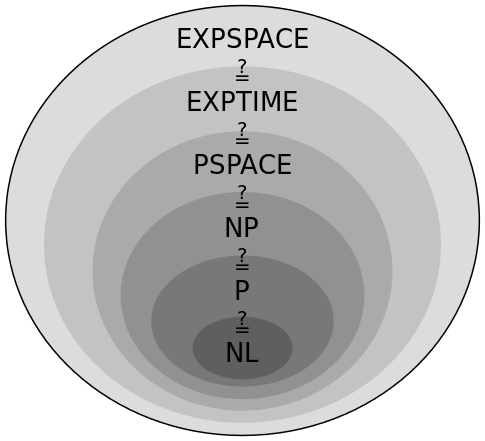
\includegraphics[width=0.5\textwidth]{img/compl.png}\blfootnote{Image from Wikipedia}
\end{figure}
\begin{align*}
LSPACE \subseteq P \subseteq NP &\subseteq PSPACE \subseteq EXPTIME \subseteq EXPSPACE \\ 
P\!\qquad\quad&\subseteq PSPACE 
\end{align*}
\end{frame}


\subsection{References}
\begin{frame}[allowframebreaks]{References}
\nocite{*} %load everything from log.bib
\bibliography{ai}
\end{frame}






\end{document}
